\section{Pillowcase homology of the pretzel knots}\label{sec:sheared}

In this section we prove Theorem~\ref{thm:hhk}. The decomposition is the one used by Hedden, Herald and Kirk
for $T(3,5)$~\cite[\S10]{HHK2}, reglued along the Conway sphere by $m=(q-5)/2$ Dehn twists. The proof has
four steps.
\begin{enumerate}
\item The reglued knot is $K_q=P(-2,3,q)$ (\S\ref{ss:decomp-P}). The argument uses only the fundamental group and the
signature and, apart from the base case (Remark~\ref{rem:chirality}), no planar diagram of the decomposition.
\item On the pillowcase the regluing replaces $L_1$ by its image under a linear shear (\S\ref{ss:shear}).
\item The unperturbed variety of the $T(3,5)$ tangle maps onto two straight polygons (\S\ref{ss:straight}). This rests
on a word in $\pi_1(Y\setminus T)$ that is trivial on the whole central circle of the variety.
\item The perturbed curves are those of~\cite{WuebbenV}, sheared (\S\ref{ss:perturbed-P}). From them we compute the
generators, the gradings and the bigons by hand (\S\S\ref{ss:gens-P}--\ref{ss:bigons-P}), for both ways in which the
perturbation can resolve the double points.
\end{enumerate}
No invariance theorem of~\cite{HHK2} is used. As in~\cite{WuebbenV}, results of~\cite{HHK2} are cited by their
numbering in arXiv:1501.00028v1.

Throughout, $\varepsilon=(\varepsilon_A,\varepsilon_B)$ denotes the parameters of the holonomy perturbation on the tangle side
((P1) in \S\ref{ss:straight}), and $\epsilon>0$ the earring parameter of \S\ref{ss:earring}. As in~\cite[\S6]{WuebbenV}, $\varepsilon$ is fixed first and $\epsilon$ is
then taken sufficiently small, and all statements about intersection points with $L_0$ hold for every
sufficiently small $\epsilon$.

\subsection{The decomposition}\label{ss:decomp-P}

\subsubsection*{The tangle}
Let $(Y,T)$ be the tangle of~\cite[\S10]{HHK2} for $T(3,5)$, with the integers $(r,s)=(2,-1)$ satisfying $3r+5s=1$;
this is the tangle of~\cite[\S3]{WuebbenV} for $n=5$. The group $\pi_1(Y\setminus T)$ is free on two elements $A,B$
(the elements $A_1,B_1$ of~\cite[\S10]{HHK2}, called $A,B$ in~\cite[\S11]{HHK1}). At $\varepsilon=0$ the meridians of the four boundary punctures are
\begin{equation}\label{eq:words-P}
a=A^2B^3,\qquad b=B^{-2}A^{-1},\qquad c=B^{-2}aB^2,
\end{equation}
by~\cite[(42)]{HHK1}, where Hedden, Herald and Kirk's torus-knot parameters are $3$ and $5$ and $(r,s)=(2,-1)$, so that the four exponents in their formula are $s+3=2$, $5-r=3$, $r=2$ and $s=-1$ (see~\cite[(3.2)]{WuebbenV}), and the fourth meridian $d$
satisfies $ba=cd$~\cite[\S3.3]{HHK1}. More generally, for $n=3\nu+2$ with $\nu\ge1$, the tangle
of~\cite[\S10]{HHK2} for $T(3,n)$ with $(r,s)=(\nu+1,-1)$ has
\begin{equation}\label{eq:words-n}
a=A^2B^{2\nu+1},\qquad b=B^{-(\nu+1)}A^{-1},\qquad c=B^{-(\nu+1)}aB^{\nu+1}.
\end{equation}

\subsubsection*{The trivial tangle and the twist}
Let $(D,U)$ be the trivial tangle of~\cite[(17)]{HHK2}: $D$ is the unit ball, and $U$ consists of the two vertical
arcs $\{(\pm1/\sqrt2,0,t):|t|\le1/\sqrt2\}$, one joining the punctures $a,d$ and the other joining $b,c$. The
group $\pi_1(D\setminus U)$ is free, and its boundary meridians satisfy $a=d$ and $b=c$~\cite[Prop.~6.1]{HHK1},
\cite[p.~4]{FKP}. Let $e\subset\partial D$ be the equator $\{z=0\}$; it separates $\{a,b\}$ from $\{c,d\}$ and bounds
the horizontal disc $D_e=D\cap\{z=0\}$, which meets each arc of $U$ once. Let $t_e$ be the Dehn twist along $e$ that
acts on $\pi_1(S^2\setminus\{a,b,c,d\})=\langle a,b,c,d\mid ba=cd\rangle$, with base point on the side of $c,d$, by
\begin{equation}\label{eq:te}
t_e(a)=(ba)\,a\,(ba)^{-1},\qquad t_e(b)=(ba)\,b\,(ba)^{-1},\qquad t_e(c)=c,\qquad t_e(d)=d .
\end{equation}
It fixes $ba=cd$. Hedden, Herald and Kirk use the half twist $g$ in the hemisphere containing $c$ and $d$ that
exchanges $c$ and $d$, and note that $g^2$ is the Dehn twist about $e$~\cite[proof of Thm.~9.2, p.~49]{HHK2}. With
base point near $a$, $g_*$ fixes $a,b$ and sends $c\mapsto d$, $d\mapsto d^{-1}cd$. So $g^2_*$ conjugates $c$ and $d$ by
$(cd)^{-1}=(ba)^{-1}$ and fixes $a,b$, and composing $(g_*^2)^{-1}$ with conjugation by $(ba)^{-1}$ gives $t_e^{-1}$.
Thus $t_e$ and $g^2$ are the same mapping class.

Recovering a knot from $(Y,T)$ requires a choice of identification of $\partial D$ with $\partial Y$~\cite[after (17)]{HHK2}.
For $h\in\Z$ let
\[
K^{(h)}=(Y,T)\cup_{t_e^h}(D,U)
\]
be the knot obtained by precomposing the identification of~\cite[(17)]{HHK2}, on the side of $Y$, with $t_e^h$: a
boundary loop $x$ of $D$ is identified with the loop $t_e^h(x)$ of $Y$.

\begin{lemma}\label{lem:group}
For every $h\in\Z$, $K^{(h)}$ is a knot in $S^3$ and
\[
\pi_1(S^3\setminus K^{(h)})\cong\langle A,B\mid t_e^h(b)=c\rangle,\qquad t_e^h(b)=(ba)^h\,b\,(ba)^{-h},
\]
with $a,b,c$ the words of the tangle. The knots $K^{(h)}$ and $K^{(h-1)}$ differ by one full twist of the two arcs
of $U$ about each other along $D_e$; in particular they are related by one crossing change.
\end{lemma}

\begin{proof}
Gluing two balls along their boundary gives $S^3$, and $t_e$ fixes each puncture, so the strands are connected as
in $K^{(0)}$, which is a knot. By van Kampen's theorem, $\pi_1(S^3\setminus K^{(h)})$ is the amalgam of
$\pi_1(Y\setminus T)=F(A,B)$ and $\pi_1(D\setminus U)$, free on $x=a=d$ and $y=b=c$, over the four-punctured sphere.
Eliminating $x$ and $y$ leaves the relations $t_e^h(b)=t_e^h(c)=c$ and $t_e^h(a)=t_e^h(d)=d$. The second follows from
the first, because $t_e^h$ fixes $ba=cd$: $t_e^h(a)=t_e^h(b)^{-1}ba=c^{-1}ba=d$. Regluing by $t_e^{-1}$ amounts to replacing
$U$ by its image under a twist map supported in a collar of $\partial D$, which is $U$ with one full twist of its two
arcs along $D_e$. Changing one of the two crossings of a full twist of two strands undoes it.
\end{proof}

At $h=0$ the relation $b=c$ reads $B^{-2}A^{-1}=B^{-2}A^2B^5$, that is $A^3B^5=1$, the group of $T(3,5)$, as it must be.

Clay and Watson define the twisted torus knots $T^m_{3,n}$ by adding $m$ positive full twists on two of the three
strands of $T(3,n)$~\cite[\S3.2]{ClayWatson}; $T^m_{3,n}$ is the closure of the braid $(\sigma_1\sigma_2)^n\sigma_1^{2m}$
(\S\ref{ss:knots}). For $n=3\nu+2$ they give the presentation~\cite[Prop.~22]{ClayWatson}
\begin{equation}\label{eq:CW}
\pi_1(S^3\setminus T^m_{3,n})\cong\bigl\langle\alpha,\beta\ \big|\ \alpha^2(\beta^{-\nu}\alpha)^m\alpha=\beta^{2\nu+1}(\beta^{-\nu}\alpha)^m\beta^{\nu+1}\bigr\rangle,
\qquad m\ge0 .
\end{equation}

\begin{lemma}\label{lem:relator}
Let $n=3\nu+2$ with $\nu\ge1$, let $(Y,T)$ be the tangle with the words~\eqref{eq:words-n}, and put $C=AB^\nu$. For every
$m\ge0$ the relation $t_e^{-m}(b)=c$ is equivalent to the vanishing of the cyclic word
\[
R_{n,m}=B^{\nu+1}A\,C^m\,A^2B^{2\nu+1}\,C^{-m},
\]
and under $\alpha=A$, $\beta=B^{-1}$ the relator of~\eqref{eq:CW} is a cyclic permutation of $R_{n,m}$. In particular
$\pi_1(S^3\setminus K^{(-m)})\cong\pi_1(S^3\setminus T^m_{3,n})$.
\end{lemma}

\begin{proof}
Since $ba=B^{-(\nu+1)}AB^{2\nu+1}=B^{-(\nu+1)}C\,B^{\nu+1}$, we have $(ba)^j=B^{-(\nu+1)}C^jB^{\nu+1}$. Hence
$t_e^{-m}(b)=B^{-(\nu+1)}C^{-m}A^{-1}B^{-(\nu+1)}C^mB^{\nu+1}$, and $t_e^{-m}(b)=c$ becomes
$C^{-m}A^{-1}B^{-(\nu+1)}C^m=A^2B^{2\nu+1}$. The inverse of the corresponding relator is
$A^2B^{2\nu+1}C^{-m}B^{\nu+1}AC^m$, a cyclic permutation of $R_{n,m}$. On the other side, substitute $\alpha=A$ and
$\beta=B^{-1}$ in the relator of~\eqref{eq:CW}:
\[
\alpha^2(\beta^{-\nu}\alpha)^m\alpha\,\beta^{-(\nu+1)}(\beta^{-\nu}\alpha)^{-m}\beta^{-(2\nu+1)}\ \longmapsto\ A^2(B^\nu A)^mA\,B^{\nu+1}(B^\nu A)^{-m}B^{2\nu+1}.
\] Using $A(B^\nu A)^m=C^mA$ and $(B^\nu A)^{-m}=B^\nu C^{-m}B^{-\nu}$, this is
$AC^mA^2B^{2\nu+1}C^{-m}B^{\nu+1}$, again a cyclic permutation of $R_{n,m}$.
\end{proof}

The group of a knot does not distinguish it from its mirror image, so the chirality of the base case enters as a
premise.

\begin{remark}[Base case]\label{rem:chirality}
The decomposition~\cite[(17)]{HHK2} gives the positive torus knot $T(3,5)$, of signature $-8$. Hedden, Herald and Kirk
call $K^{(0)}$ the $(3,5)$ torus knot without fixing its handedness~\cite[\S10]{HHK2}, and their comparison
in~\cite[\S11]{HHK2} uses $\sigma$ only modulo $4$, so it does not decide the question; the knot group cannot detect it
either. We verify it by a computer-assisted argument. From a planar diagram of~\cite[Fig.~18]{HHK2}, SnapPy~\cite{SnapPy},
with verified computation of canonical cell decompositions by interval arithmetic~\cite{HIKMOT,DHL}, shows that the
complement of the link $K^{(0)}\cup e$ is isometric to the complement of the closure of the positive braid
$(\sigma_1\sigma_2)^5$ together with an unknotted circle encircling two of its strands, and that every such isometry
preserves the orientation and the meridians (Appendix~\ref{app:data}). Such an isometry extends to an
orientation-preserving homeomorphism of $S^3$ carrying $K^{(0)}$ to the closure of $(\sigma_1\sigma_2)^5$, the positive torus
knot. The identification of the knots below and the graded comparison in Theorem~\ref{thm:hhk} rest on this.
\end{remark}

\begin{theorem}\label{thm:topology}
For every $m\ge1$, the knot $K^{(-m)}$ is the pretzel knot $K_{5+2m}=P(-2,3,5+2m)$, the closure of the positive braid
$(\sigma_1\sigma_2)^5\sigma_1^{2m}$, and $\sigma(K^{(-m)})=-(2m+6)$.
\end{theorem}

\begin{proof}
By Lemma~\ref{lem:relator} with $\nu=1$, the groups of $K^{(-m)}$ and of $T^m_{3,5}$ are isomorphic. Clay and Watson state
that $T^m_{3,5}$ is $P(-2,3,5+2m)$~\cite[\S3.2]{ClayWatson}; for $m=1$ this is also stated in~\cite[p.~164]{DS24}. We use
this only up to mirror image. In particular both knots are nontrivial, since the Alexander polynomial of their common
group is that of $K_{5+2m}$, which is not constant (Lemma~\ref{lem:alex}). Both groups are generated by two elements, so
both knots are prime by Norwood's theorem~\cite{Norwood}. Prime knots with isomorphic groups are equivalent, by a
homeomorphism of $S^3$ that may reverse orientation~\cite[Cor.~2.1]{GordonLuecke}. Hence $K^{(-m)}$ is $K_{5+2m}$ or its
mirror image.

To fix the chirality, recall $\sigma(K_q)=-(q+1)$ for $q\ge7$ and $\sigma(K_5)=\sigma(T(3,5))=-8$
(Proposition~\ref{prop:sig}); the mirror image has the opposite signature. By Lemma~\ref{lem:group}, $K^{(-m-1)}$ and
$K^{(-m)}$ are related by one crossing change, so their signatures differ by at most $2$~\cite[proof of Thm.~10.1, (10.2)]{Murasugi}.
Suppose $\sigma(K^{(-m)})=-s_m$ with $s_0=8$ and $s_m=2m+6$ for $m\ge1$; for $m=0$ this is Remark~\ref{rem:chirality}.
The two candidates for $K^{(-m-1)}$ have signature $\pm(2m+8)$, and only $-(2m+8)$ lies within $2$ of $-s_m$. Hence
$K^{(-m-1)}=K_{2m+7}$, and induction on $m$ shows $K^{(-m)}=K_{5+2m}$ for every $m\ge1$.

It remains to see that $K_{5+2m}$, rather than its mirror image, is the closure of $(\sigma_1\sigma_2)^5\sigma_1^{2m}$. By
Clay and Watson, used up to mirror image, this closure is $K_{5+2m}$ or its mirror image. Changing one crossing of
$\sigma_1^{2m}$ from positive to negative gives $(\sigma_1\sigma_2)^5\sigma_1^{2m-2}$, and for knots $K_\pm$
related by such a change $\sigma(K_+)-\sigma(K_-)\in\{0,-2\}$ in our convention (see the proof of
Proposition~\ref{prop:twisted-sig}). By induction from $\sigma(T(3,5))=-8$, the closure has negative signature. Since
$\sigma(K_{5+2m})=-(2m+6)<0$ and its mirror image has positive signature, the closure is $K_{5+2m}$.
\end{proof}

The same argument applies to every $n\equiv2\pmod3$ once the signature of $T(3,n;2,m)$ is known; this is used in
Section~\ref{sec:twisted}.

\begin{proposition}\label{prop:hyperbolic}
For odd $q\ge7$ the knot $K_q$ is hyperbolic and is not a two-bridge knot.
\end{proposition}

\begin{proof}
By Lemma~\ref{lem:not-torus}, $K_q$ is neither two-bridge nor a torus knot. It is the Montesinos knot with rational
tangles $-1/2$, $1/3$, $1/q$, all of denominator at least $2$. By Oertel's theorem~\cite[Cor.~5]{Oertel}, the
complement of such a Montesinos link carries a complete hyperbolic structure unless the link is a torus link or one
of the links $K(\tfrac12,\tfrac12,-\tfrac12,-\tfrac12)$, $K(\tfrac23,-\tfrac13,-\tfrac13)$, $K(\tfrac12,-\tfrac14,-\tfrac14)$,
$K(\tfrac12,-\tfrac13,-\tfrac16)$ or a mirror image of one of these. For each of the four listed links the sum of the
fractions is $0$. The determinant of a Montesinos link with fractions $\beta_i/\alpha_i$ is
$|\alpha_1\cdots\alpha_r\sum_i\beta_i/\alpha_i|$, the order of the first homology of its double branched cover (infinite,
and the determinant $0$, when the sum vanishes), whereas the determinant of a knot is odd; so none of them, and none
of their mirror images, is a knot. Conventions for the sign of a rational tangle differ between authors, which may replace $K_q$ by its
mirror image; the list of exceptions is closed under mirror image. Hence $K_q$ is hyperbolic.
\end{proof}

Oertel's corollary does not list the torus links, which is why Lemma~\ref{lem:not-torus} is needed. Explicitly,
apart from two-bridge knots the only non-hyperbolic Montesinos knots are $P(-2,3,3)=T(3,4)$ and $P(-2,3,5)=T(3,5)$
and their mirror images~\cite[Rem.~1]{IchiharaJong},~\cite[p.~440]{Meier}. Futer and Gu\'eritaud give a published
proof of the classification of non-hyperbolic arborescent links, which they attribute to Bonahon and
Siebenmann~\cite[Thm.~1.5]{FutGue}.

\subsection{The twist acts by a shear}\label{ss:shear}

For $h\in\Z$ let $S_h\colon\R^2\to\R^2$ be the linear map $S_h(\gamma,\theta)=(\gamma,\theta-2h\gamma)$.

\begin{lemma}\label{lem:shear}
Let $(Y,T)$ be a $2$-tangle as in~\cite[(17)]{HHK2}, with a holonomy perturbation supported in the interior of $Y$, and
let $h\in\Z$. For the decomposition $(Y,T)\cup_{t_e^h}(D,U)$:
\begin{enumerate}
\item[(a)] $R_\pi(Y,T)$ is unchanged, its restriction map is $S_h\circ L_1$, where $L_1$ is the restriction map for the
identification of~\cite[(17)]{HHK2}, and $L_0$ is unchanged;
\item[(b)] $S_h$ descends to a homeomorphism of $P$ fixing each corner and to an orientation-preserving
diffeomorphism of $\Pst$; it preserves $\gamma$, hence the open strip $\{0<\gamma<\pi\}$, the two edges, and the vertical
degree of closed curves that miss the edges;
\item[(c)] $S_h$ maps proper immersions of intervals to proper immersions, adding $-2h$ to both limiting slopes, and
preserves embeddedness of lifts and the absence of fishtails;
\item[(d)] for closed curves $S_h$ preserves $z$ and $\mu(\cdot,\ell_1)$; hence it maps restricted immersed
$1$-manifolds to restricted immersed $1$-manifolds;
\item[(e)] the corner images of the two abelian representations are unchanged;
\item[(f)] for every immersed path $\alpha$, $\mu(S_h\circ\alpha,\ell_1)=\mu(\alpha,S_h^{-1}\ell_1)$, where $S_h^{-1}\ell_1$ is the
constant line field spanned by $(1,1+2h)$.
\end{enumerate}
\end{lemma}

\begin{proof}
(a) The perturbation is supported in the interior of $Y$, so $R_\pi(Y,T)$ does not change. Let a representation
restrict to $a\mapsto\mathbf i$, $b\mapsto e^{\gamma\mathbf k}\mathbf i$, $c\mapsto e^{\theta\mathbf k}\mathbf i$ on $\partial Y$. Then
$\rho(ba)=-e^{\gamma\mathbf k}$, so by~\eqref{eq:te}, $\rho(t_e^ha)=e^{2h\gamma\mathbf k}\mathbf i$, $\rho(t_e^hb)=e^{(2h+1)\gamma\mathbf k}\mathbf i$,
and $c$ is fixed. Conjugating by $e^{-h\gamma\mathbf k}$ gives $(\mathbf i,\ e^{\gamma\mathbf k}\mathbf i,\ e^{(\theta-2h\gamma)\mathbf k}\mathbf i)$, the
point $S_h(\gamma,\theta)$, with $\gamma\in[0,\pi]$ unchanged. The trivial tangle keeps the identification
of~\cite[(17)]{HHK2}, so $L_0$ is unchanged.

(b) $S_h$ is linear of determinant $1$ and commutes with $-1$; it sends $(2\pi,0)$ to $(2\pi,-4\pi h)$ and fixes
$(0,2\pi)$, so it normalizes $G$. It maps $(\pi a,\pi b)$ to $(\pi a,\pi(b-2ha))\equiv(\pi a,\pi b)$ modulo $2\pi\Z^2$.

(c) Embeddedness of lifts and the absence of fishtails are invariant under the homeomorphism $S_h$ of $\Pst$.

(d) $S_h$ fixes the corners and preserves orientation, so it preserves $z$. For a closed curve, $\mu(\cdot,\ell)$ is
the total rotation of the tangent line divided by $\pi$, for every constant line field $\ell$, because the deck
transformations have derivative $\pm I$. Along the path $s\mapsto S_{sh}$, $0\le s\le1$, this total rotation is a
continuous integer, hence constant. The rest follows from (b), (c) and Definition~\ref{def:restricted}.

(e) This follows from (b).

(f) The tangent line of $S_h\circ\alpha$ equals $\ell_1$ exactly when the tangent line of $\alpha$ equals $S_h^{-1}\ell_1$. Since
$S_h$ preserves orientation, the senses of passage agree, and the endpoint conventions correspond.
\end{proof}

The computation in (a) is that of~\cite[(28)]{HHK2}: there the half twist $g$ acts on the pillowcase by
$(\gamma,\theta)\mapsto(\gamma,\theta-\gamma)$, and~\cite[(29)--(30)]{HHK2} obtain the action of $\mathrm{PSL}_2(\Z)$ from $g$ and a
$3$-cycle. Since $t_e=g^2$, $t_e^h$ acts by $S_h$. Our additions are the observation that regluing by $t_e^h$ is a
choice of identification permitted by~\cite[(17)]{HHK2}, and properties (b)--(f). The action of the mapping class
group on the pillowcase is also~\cite[Thm.~B]{CHK}, and its counterpart for immersed curves in Khovanov
homology is~\cite[Thm.~8.1]{KWZ}.

\subsubsection*{The pretzel case}
From now on $q\ge7$ is odd and $m=(q-5)/2$, so that
\[
S_{-m}(\gamma,\theta)=\bigl(\gamma,\ \theta+(q-5)\gamma\bigr).
\]
By Theorem~\ref{thm:topology} and Lemma~\ref{lem:shear}, the decomposition $K_q=(Y,T)\cup_{t_e^{-m}}(D,U)$ has restriction
map $S_{-m}\circ L_1$, where $L_1$ is the restriction map of~\cite{WuebbenV} for $T(3,5)$. On $\R^2$ we keep
$\varphi=\theta-\gamma$; then
\[
\varphi\circ S_{-m}=\lambda,\qquad \lambda(\gamma,\theta)=\theta+(q-6)\gamma ,
\]
and $S_{-m}^{-1}\ell_1$ is the line field spanned by $(1,6-q)$.

\subsection{The unperturbed curve}\label{ss:straight}

We use the following facts about the tangle $(Y,T)$ for $n=5$ and its holonomy perturbations, in the notation
of~\cite[\S\S3--6]{WuebbenV} with these changes: the perturbation parameters, written $\epsilon=(\epsilon_A,\epsilon_B)$
there, are written $\varepsilon=(\varepsilon_A,\varepsilon_B)$ here; the binary dihedral arc $B$ of~\cite{WuebbenV}, its
pieces $B_0,B_1,B_2$ and the vectors $T_B$, $P_B$ are written $\Omega$, $\Omega_0,\Omega_1,\Omega_2$, $T_\Omega$, $P_\Omega$, to
distinguish them from the generator $B$; the lines $\Delta_k$ and the strands $S^k_\pm$ of~\cite{WuebbenV} are the lines
$\mathcal D_k$ and the lifts $S^k_\pm$ of $L_0$ of \S\ref{ss:earring}; and the reduced function $g$
of~\cite[\S5.2]{WuebbenV} is written $f_c$.
\begin{enumerate}
\item[(P1)] \emph{The perturbation}~\cite[\S3.1]{WuebbenV}. The group $\pi_1(Y\setminus T)$ is free on $A,B$, and the
holonomy perturbation $\pi$ is supported near two curves $P_A,P_B$ in $Y$, those of~\cite[\S10]{HHK2}, with
perturbation functions $\varepsilon_A\sin$ and $\varepsilon_B\sin$. A perturbed traceless representation is determined, up
to conjugation, by
\[
A\mapsto e^{uQ_A},\qquad B\mapsto e^{vQ_B},\qquad Q_A=\mathbf i,\qquad Q_B=\tau\,\mathbf i+\sqrt{1-\tau^2}\,\mathbf j,
\]
with $(u,v,\tau)\in[0,\pi]^2\times[-1,1]$.
\item[(P2)] \emph{The equations}~\cite[\S3.1 and Lemma~3.1]{WuebbenV},~\cite[(33)--(34)]{HHK2}. The meridians $a,b$ of
$T$ are sent to traceless elements exactly when $\Psi=(\Psi_1,\Psi_2)=0$, where
$\Psi_i=\cos\Theta_i\cos\Phi_i-\tau\sin\Theta_i\sin\Phi_i$ and, for $n=5$, the perturbed phases are
\[
\Phi_1=2u+3\varepsilon_A\sin u,\qquad \Theta_1=3v-2\varepsilon_B\sin v,\qquad \Phi_2=-u-2\varepsilon_A\sin u,\qquad
\Theta_2=-2v+\varepsilon_B\sin v .
\]
Put $W_\varepsilon=\Psi(\varepsilon;\cdot)^{-1}(0)\subset[0,\pi]^2\times[-1,1]$ and $W=W_0$. There is a surjection
$W_\varepsilon\to R_\pi(Y,T)$~\cite[Thm.~10.2]{HHK2}, whose fiber over the image of $(u,v,\tau)$ is that single point unless
$\sin u=0$ or $\sin v=0$, in which case it is the segment $\{(u,v)\}\times[-1,1]$. At $\varepsilon=0$,
$\Psi=(\mathrm{E2},\mathrm{E1})$, where (E1) and (E2) denote
\[
\cos2v\cos u-\tau\sin2v\sin u\qquad\text{and}\qquad\cos3v\cos2u-\tau\sin3v\sin2u .
\]
The restriction map $\Pi=\Pi_\varepsilon\colon W_\varepsilon\to P$ is normalized by $a\mapsto\mathbf i$,
$b\mapsto e^{\gamma\mathbf k}\mathbf i$, $c\mapsto e^{\theta\mathbf k}\mathbf i$ with $\gamma\in[0,\pi]$, and it depends smoothly on
$(\varepsilon,u,v,\tau)$ where it is defined~\cite[\S\S3.1, 5]{WuebbenV}.
\end{enumerate}
The unperturbed variety $W$ is described as follows.
\begin{enumerate}
\item[(V1)] $W=\Omega\cup C_0$, where $\Omega=\{(\frac\pi2,\frac\pi2)\}\times[-1,1]$ is the binary dihedral arc and $C_0$ is the central
circle; $C_0\cap \Omega=\{c_+,c_-\}$ with $c_\pm=(\frac\pi2,\frac\pi2,\pm\tau_1)$, $\tau_1=\sqrt3/2$; the halves
$C_0^{\mathrm L}=C_0\cap\{v\le\frac\pi2\}$ and $C_0^{\mathrm R}=C_0\cap\{v\ge\frac\pi2\}$ meet $\{v=\frac\pi2\}$ only at $c_\pm$
\cite[Prop.~3.6, Prop.~3.10(2)]{WuebbenV}.
\item[(V2)] $\Pi(\Omega)$ lifts to the segment $t\mapsto(t,0)$, $t\in[0,\pi]$, with $\gamma=\arccos\tau$ on $\Omega$. The endpoints
$r_\pm=(\frac\pi2,\frac\pi2,\pm1)$ map to $(0,0)$ and $(\pi,0)$, and $\Pi(c_+)=(\frac\pi6,0)$, $\Pi(c_-)=(\frac{5\pi}6,0)$
\cite[Prop.~3.9]{WuebbenV}. We write $\Omega_0$, $\Omega_1$, $\Omega_2$ for the pieces of $\Omega$ with $\tau\in[\tau_1,1]$,
$[-\tau_1,\tau_1]$, $[-1,-\tau_1]$.
\item[(V3)] Along each half of $C_0$, from $c_+$ to $c_-$, $\varphi$ is strictly monotone with $d\varphi\neq0$ at interior
points and increases by $10\pi/3$; at interior points $\frac\pi6<\gamma<\frac{5\pi}6$~\cite[Thm.~4.10,
Props.~4.11--4.12]{WuebbenV}.
\item[(V4)] $v$ is a regular parameter of $C_0$ at $c_\pm$, and on a lift
$\Pi=\Pi(c_\pm)\pm V_0(v-\frac\pi2)^2+O(|v-\frac\pi2|^3)$ with $V_0=(2/\sqrt3,\,12/\sqrt3)$, of slope
$6$~\cite[Lemma~4.13]{WuebbenV}.
\item[(V5)] $c_\pm$ are nondegenerate double points of $W$. With respect to the equations (E1), (E2) of (P2), the
kernel of $d\Psi(c_\pm)$ is spanned by $T_\Omega=\partial_\tau$ and $X=-2\tau\partial_u+\partial_v$, the
covector $\ell=(-2\tau,-1)$ spans the left kernel, $\ell\cdot D^2\Psi(T_\Omega,X)=-8\tau$ and $\ell\cdot D^2\Psi(T_\Omega,T_\Omega)=0$
\cite[Prop.~3.11(2)]{WuebbenV}.
\end{enumerate}

\begin{lemma}\label{lem:straight}
Let $\varepsilon=0$ and put $w=(ba)^{-3}c\,(ba)^3a\in\pi_1(Y\setminus T)$. Then $\rho(w)=1$ for every $\rho\in C_0$. Consequently
$\theta\equiv6\gamma-\pi\pmod{2\pi}$ on $\Pi(C_0)$, and for $l\in\Z$ the lift of each half of $C_0$ that starts at the point
$(\frac\pi6,2\pi l)$ over $\Pi(c_+)$ is the segment
\[
\{(\gamma,\,6\gamma-\pi+2\pi l):\ \tfrac\pi6\le\gamma\le\tfrac{5\pi}6\},
\]
traversed with $\gamma$ strictly increasing from $c_+$ to $c_-$ and with $d\gamma\neq0$ at interior points.
\end{lemma}

\begin{proof}
We write quaternions as $p=p_0+\mathbf p$ with $p_0=\operatorname{Re}p$, so that $\mathbf p\mathbf q=-\mathbf p\cdot\mathbf q+\mathbf p\times\mathbf q$ for
pure quaternions.

\emph{Step 1: the word.} By~\eqref{eq:words-P}, $ba=B^{-2}(AB)B^2$, so $(ba)^3=B^{-2}w_0$ with $w_0=(AB)^3B^2$. Since
$c=B^{-2}aB^2$, we get $w=w_0^{-1}B^2\cdot B^{-2}aB^2\cdot B^{-2}w_0\cdot a=w_0^{-1}aw_0a$. If $\rho(a)$ and $\rho(w_0)$ are
orthogonal pure unit quaternions, they anticommute, so $\rho(w_0)^{-1}\rho(a)\rho(w_0)=-\rho(a)$ and $\rho(w)=-\rho(a)^2=1$. It remains to
prove that orthogonality.

\emph{Step 2: notation.} Let $\rho\in W$. Then $\beta=\rho(b)$ is a pure unit quaternion. Write $N=\rho(B)=\cos v+\sin v\,Q$
with $Q=Q_B$, and put
\[
\zeta=\beta\cdot Q,\qquad U=\cos v\,\beta+\sin v\,(\beta\times Q),\qquad E=4\cos^2v+4\zeta^2\sin^2v-3 .
\]
From $b=B^{-2}A^{-1}$ we get $\rho(A)=-\beta N^{-2}$.

\emph{Step 3: $\rho(a)$.} Conjugation by $\beta$ is the rotation by $\pi$ about $\beta$, so $\beta Q\beta^{-1}=Q'$ with $Q'=2\zeta\beta-Q$,
and $\beta N^{-2}\beta=-e^{-2vQ'}$. Hence $\rho(a)=\rho(A)^2N^3=-e^{-2vQ'}N$. Using
$\operatorname{Re}(e^{sP}e^{tR})=\cos s\cos t-(P\cdot R)\sin s\sin t$ and $Q'\cdot Q=2\zeta^2-1$,
\[
\operatorname{Re}\rho(a)=-\cos v\cdot E,\qquad \mathbf{Vec}\,\rho(a)=-\sin3v\,Q+2\zeta\sin2v\,U .
\]

\emph{Step 4: $C_0\subset\{E=0\}$.} On $W$ the element $\rho(a)$ is traceless, so $\cos v\cdot E=0$. On $C_0\setminus\{c_\pm\}$
we have $v\neq\frac\pi2$ by (V1), so $E=0$ there, and by continuity on all of $C_0$.

\emph{Step 5: $\rho(w_0)$.} Put $\xi=\beta N^{-1}$, so that $\rho(AB)=-\xi$ and $\operatorname{Re}\xi=\zeta\sin v$. The Cayley--Hamilton
identity $\xi^2=2(\operatorname{Re}\xi)\xi-1$ gives $\xi^3=(4\zeta^2\sin^2v-1)\xi-2\zeta\sin v$, and $\xi N^2=\beta N$, so
\[
\rho(w_0)=-\xi^3N^2=-(4\zeta^2\sin^2v-1)\,\beta N+2\zeta\sin v\,N^2,\qquad \operatorname{Re}\rho(w_0)=\zeta\sin v\cdot E .
\]
On $\{E=0\}$ we have $4\zeta^2\sin^2v-1=-2\cos2v$, so $\rho(w_0)$ is pure, with $\mathbf{Vec}\,\rho(w_0)=2\cos2v\,U+2\zeta\sin v\sin2v\,Q$.

\emph{Step 6: orthogonality.} On $\{E=0\}$, with $\mathbf{Vec}\,\rho(w_0)$ in the form of Step~5, and with $U\cdot U=1-\zeta^2\sin^2v$, $U\cdot Q=\zeta\cos v$ and $\sin3v=\sin v\,(4\cos^2v-1)$, a direct
expansion gives
\[
\mathbf{Vec}\,\rho(w_0)\cdot\mathbf{Vec}\,\rho(a)=2\zeta\bigl(2\zeta^2\sin^2v\sin2v+2\cos2v\sin2v-\sin3v\cos v\bigr)=\zeta\sin2v\cdot E .
\]
So on $C_0$ the quaternions $\rho(a)$ and $\rho(w_0)$ are orthogonal pure units, and $\rho(w)=1$ by Step~1.

\emph{Step 7: the pillowcase.} In the normalization of $\Pi$, $\rho(ba)=-e^{\gamma\mathbf k}$ and $\mathbf ie^{t\mathbf k}=e^{-t\mathbf k}\mathbf i$, so
$\rho\bigl((ba)^jc(ba)^{-j}a\bigr)=-e^{(\theta+2j\gamma)\mathbf k}$. For $j=-3$, $\rho(w)=1$ gives $\theta-6\gamma\in\pi+2\pi\Z$.

\emph{Step 8: the lifts.} By (V3) the lift of a closed half starting at a lift $(\frac\pi6,2\pi l)$ of $\Pi(c_+)$ stays
in the open strip except at its ends. On it $\theta-6\gamma+\pi$ is continuous with values in $2\pi\Z$, hence equal to its
value $2\pi l$ at the start, so $\varphi=5\gamma-\pi+2\pi l$. By (V3), $\varphi$ is strictly monotone with $d\varphi\neq0$ at interior
points and increases by $10\pi/3$; hence $\gamma=(\varphi+\pi-2\pi l)/5$ increases strictly from $\frac\pi6$ to $\frac{5\pi}6$,
with $d\gamma\neq0$ at interior points.
\end{proof}

Each displayed identity of Steps 1--7 has also been verified symbolically for indeterminate $(v,\zeta)$ (see
Appendix~\ref{app:data}). Hedden, Herald and Kirk observed, by a computer algebra computation, that the two halves of
the central circle for $T(3,5)$ map linearly with slope $6$~\cite[\S11.7, p.~59]{HHK2}; Lemma~\ref{lem:straight} proves
this. For their own decomposition of the pretzel knots $P(p,q,r)$ with $p$ even, Fukumoto, Kirk and Pinz\'on-Caicedo
prove the analogous straightness~\cite[Thm.~5.1]{FKP}, and they describe the unperturbed curve as the segments
$\theta=(r-5)\gamma$ and $\theta=(r+1)\gamma+\pi$~\cite[\S5, p.~28]{FKP}. These are the images under $S_{-m}$ of $\Pi(\Omega)$ and of the line
of Lemma~\ref{lem:straight}, with $r=q$. We do not identify their decomposition with ours, and we do not use their
result; we regard it as the antecedent of Lemma~\ref{lem:straight}.

By (P6) in \S\ref{ss:perturbed-P}, after a small perturbation the arc of $L_1$ is built from $\Omega_0$, one half of
$C_0$ and $\Omega_2$, possibly through $\Omega_1$ and the other half. Write $H$ for the half joined to $\Omega_0$ and $H'$ for the
other half, and orient both from $c_+$ to $c_-$. Let $O=(0,0)$, and
\[
J_1=(\tfrac\pi6,0),\quad J_2=(\tfrac{5\pi}6,4\pi),\quad J_3=(\tfrac\pi6,4\pi),\quad J_4=(\tfrac{5\pi}6,8\pi),\quad Z=(\pi,8\pi),\quad Z'=(\pi,4\pi).
\]

\begin{corollary}\label{cor:polygon}
At $\varepsilon=0$ the lifted pieces are straight segments, traversed monotonically and regular in their interiors:
$\Omega_0\colon O\to J_1$ along $(1,0)$; $H\colon J_1\to J_2$ along $(1,6)$; $\Omega_1^{-1}\colon J_2\to J_3$ along $(-1,0)$;
$H'\colon J_3\to J_4$ along $(1,6)$; and $\Omega_2\colon J_4\to Z$, or $\Omega_2\colon J_2\to Z'$ when $\Omega_2$ follows $H$, along $(1,0)$.
The lift of the closed curve $\Omega_1^{-1}\cdot H'$ is the $(0,4\pi)$-periodic polygon with vertices $(\frac{5\pi}6,4\pi j)$ and
$(\frac\pi6,4\pi j)$, $j\in\Z$.
\end{corollary}

\begin{proof}
The pieces of $\Omega$ are described by (V2): $\gamma=\arccos\tau$ is a diffeomorphism from $(-1,1)$ onto $(0,\pi)$. The halves are described by Lemma~\ref{lem:straight}, applied to the lifts starting at $J_1=(\frac\pi6,0)$ and $J_3=(\frac\pi6,4\pi)$, whose endpoints are the listed vertices.
\end{proof}

\begin{figure}[ht]
\centering
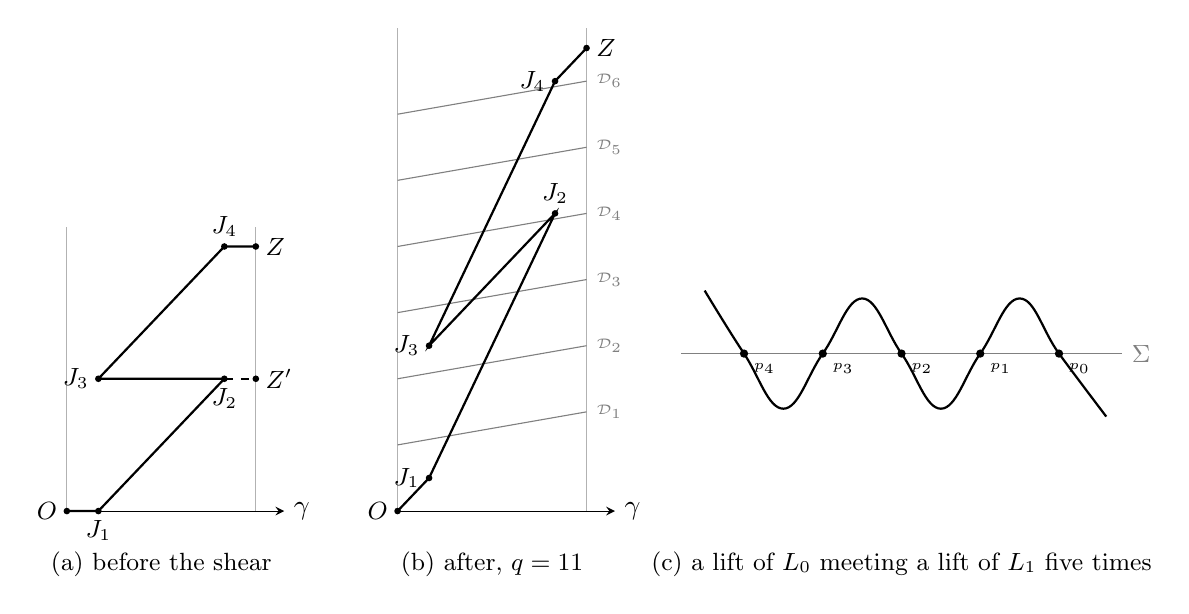
\begin{tikzpicture}[x=2.4cm,y=0.42cm,>=stealth]
% (a) unsheared polygon, theta in units of pi
\begin{scope}
\draw[gray!60] (0,0) -- (0,8.6); \draw[gray!60] (1,0) -- (1,8.6);
\draw[->] (0,0) -- (1.15,0) node[right] {$\gamma$};
\draw[thick] (0,0) -- (1/6,0) -- (5/6,4) -- (1/6,4) -- (5/6,8) -- (1,8);
\draw[thick,dashed] (5/6,4) -- (1,4);
\foreach \p/\l/\a in {{(0,0)}/O/left,{(0.1667,0)}/J_1/below,{(0.8333,4)}/J_2/below,{(0.1667,4)}/J_3/left,{(0.8333,8)}/J_4/above,{(1,8)}/Z/right,{(1,4)}/Z'/right}
  \fill \p circle (1.2pt) node[\a] {\small$\l$};
\node at (0.5,-1.6) {\small(a) before the shear};
\end{scope}
% (b) sheared polygon for q=11 (shear 6), with lines D_k
\begin{scope}[xshift=4.2cm]
\draw[gray!60] (0,0) -- (0,14.6); \draw[gray!60] (1,0) -- (1,14.6);
\draw[->] (0,0) -- (1.15,0) node[right] {$\gamma$};
\foreach \k in {1,...,6} \draw[gray] (0,2*\k) -- (1,2*\k+1) node[right] {\tiny$\mathcal D_{\k}$};
\draw[thick] (0,0) -- (1/6,1) -- (5/6,9) -- (1/6,5) -- (5/6,13) -- (1,14);
\foreach \p/\l/\a in {{(0,0)}/O/left,{(0.1667,1)}/J_1/left,{(0.8333,9)}/J_2/above,{(0.1667,5)}/J_3/left,{(0.8333,13)}/J_4/left,{(1,14)}/Z/right}
  \fill \p circle (1.2pt) node[\a] {\small$\l$};
\node at (0.5,-1.6) {\small(b) after, $q=11$};
\end{scope}
% (c) chain schematic
\begin{scope}[xshift=8.6cm,yshift=2cm,x=1cm,y=1cm]
\draw[gray] (-0.8,0) -- (4.8,0) node[right] {\small$\Sigma$};
\draw[thick] plot[smooth,tension=0.7] coordinates {(4.6,-0.8) (4,0) (3.5,0.7) (3,0) (2.5,-0.7) (2,0) (1.5,0.7) (1,0) (0.5,-0.7) (0,0) (-0.5,0.8)};
\foreach \x/\i in {4/0,3/1,2/2,1/3,0/4} \fill (\x,0) circle (1.5pt) node[below right] {\tiny$p_{\i}$};
\node at (2,-2.67) {\small(c) a lift of $L_0$ meeting a lift of $L_1$ five times};
\end{scope}
\end{tikzpicture}
\caption{(a) The lift of the unperturbed curve for $T(3,5)$, at $\varepsilon=0$ (Corollary~\ref{cor:polygon}); the dashed segment is $\Omega_2$
when it follows $H$. Vertical units are multiples of $\pi$. (b) Its image under $S_{-m}$ for $q=11$, with the lines $\mathcal D_k$;
the lines $\mathcal D_3$ and $\mathcal D_4$ are crossed three times. (c) The configuration of Lemma~\ref{lem:zigzag}: the points
$p_0,\dots,p_4$ are ordered by decreasing $\gamma$, and the lobes alternate above and below the lift $\Sigma$ of $L_0$.}
\label{fig:sheared}
\end{figure}

\subsection{The perturbed curves}\label{ss:perturbed-P}

Besides (P1) and (P2) we use the following results of~\cite[\S\S5--6]{WuebbenV}, stated for $n=5$. In them $c$
is one of the double points $c_\pm$ of (V1), $\ell$ is the covector of (V5), and $L_1$ and $\tilde A$ are the curve
of~\cite{WuebbenV} and its lift, before the shear; statements that involve $L_0$ hold, as in~\cite[\S6]{WuebbenV}, for
$\varepsilon\in\mathcal C_a$ sufficiently small and then every sufficiently small earring parameter.
\begin{enumerate}
\item[(P3)] \emph{The reduced function}~\cite[\S5.2]{WuebbenV}. The differential $d\Psi(c)$ has rank one, its kernel is
spanned by $T_\Omega$ and the tangent $T_C$ of $C_0$ at $c$, and the restriction of $\ell\cdot D^2\Psi(c)$ to $\ker d\Psi(c)$ is
a nondegenerate indefinite quadratic form~\cite[Prop.~3.11]{WuebbenV}. In coordinates $(s,t,\varrho)$ centered at $c$
with $\partial_s=T_\Omega$ and $\partial_t=T_C$ at $c$, for a covector $m$ not proportional to $\ell$ the function $m\cdot\Psi$ has nonzero $\partial_\varrho$-derivative at $c$ and can be solved for
$\varrho=\varrho(s,t,\varepsilon)$ by the implicit function theorem, and near $c$ the variety $W_\varepsilon$ is the zero set of the
\emph{reduced function}
\[
f_c(s,t;\varepsilon)=\ell\cdot\Psi\bigl(\varepsilon;s,t,\varrho(s,t,\varepsilon)\bigr),
\]
that is, of the Lyapunov--Schmidt reduction of $\Psi$ to $\ker d\Psi(c)$; its Hessian at $(0,0;0)$ is the quadratic form
above. For small $\varepsilon$ the function $f_c(\cdot;\varepsilon)$ has a unique critical point near $0$, depending
analytically on $\varepsilon$, with critical value $\kappa_c(\varepsilon)$, and there are coordinates $(s',t')$, depending
analytically on $\varepsilon$, with $f_c=\kappa_c(\varepsilon)+s't'$; at $\varepsilon=0$ they are chosen so that $\{t'=0\}$ is
$\Omega$ and $\{s'=0\}$ is $C_0$ near $c$. Moreover $\kappa_c(0)=0$ and $d\kappa_c(0)=\ell\cdot\partial_\varepsilon\Psi(0;c)$.
\item[(P4)] \emph{The cone}~\cite[Def.~5.5]{WuebbenV}. For $a>0$, $\mathcal C_a$ is the set of $\varepsilon\in\R^2$ such that
the linear part $d\kappa_c(0)\varepsilon$ of $\kappa_c(\varepsilon)$ has absolute value at least $a|\varepsilon|$ at both double points $c=c_\pm$, for the covector $\ell$ of (V5); another normalization of $\ell$ rescales $a$.
\item[(P5)] \emph{Near the double points}~\cite[Lemma~5.6 and its proof]{WuebbenV}. Let $P_\Omega$ and $V$ be the vectors
with $\Pi(s',0)=\Pi(c)+s'P_\Omega+O(s'^2)$ and $\Pi(0,t')=\Pi(c)+t'^2V+O(t'^3)$ at $\varepsilon=0$; they are linearly
independent. Let $a>0$. There are $r_1>0$ and constants $C,c_0>0$ such that for every $r_0\in(0,r_1]$ there is $\varepsilon_0>0$ with the following properties for every $\varepsilon\in\mathcal C_a$ with $0<|\varepsilon|<\varepsilon_0$. Let $U_c$ be the set of points of a fixed neighborhood of $c$
whose coordinates $(s,t)$ have Morse coordinates $(s',t')$ with $|s'|\le r_0$ and $|t'|\le r_0$; it depends on
$\varepsilon$, but it contains and is contained in fixed neighborhoods of $c$. Each of the two arcs of $W_\varepsilon\cap U_c$
is mapped by $\Pi$ to an embedded arc with nowhere vanishing velocity. Such an arc is parametrized by $t'$, with
$s'=-\kappa/t'$, $\kappa=\kappa_c(\varepsilon)$ and $|\kappa|/r_0\le|t'|\le r_0$, and its velocity is
\[
\frac{d}{dt'}\Pi_\varepsilon=\frac{\kappa}{t'^2}P_\Omega+2t'V+e(t'),\qquad
|e(t')|\le C\bigl(r_0+|\varepsilon|^{2/3}a^{-1/3}\bigr)A(t'),\qquad A(t')=\frac{|\kappa|}{t'^2}+|t'|,
\]
with $C$ independent of $\varepsilon$, $a$ and $r_0$; the main term $(\kappa/t'^2)P_\Omega+2t'V$ has length at least $c_0A(t')$.
\item[(P6)] \emph{Global structure}~\cite[Prop.~5.7(1), (2), (4)]{WuebbenV}. Let $a>0$. For every
$\varepsilon\in\mathcal C_a$ with $0<|\varepsilon|$ sufficiently small, $R_\pi(Y,T)$ is a compact $1$-manifold with two
boundary points $r_\pm(\varepsilon)$, and $L_1$ is an immersion into $\Pst$ away from $r_\pm(\varepsilon)$. Away from
$U_{c_\pm}$ and from the corner charts of (P7), $W_\varepsilon$ is $C^1$-close to $W$: it is the image of a $C^1$-small
normal graph over $W$, with $\Pi_\varepsilon$ correspondingly $C^1$-close to $\Pi$. The union $\Omega\cup C_0$ is replaced by its
resolution at the two double points: either the arc is $\Omega_0\cdot C_0^{\mathrm X}\cdot\Omega_2$ and there is one further
circle $\Omega_1\cdot(C_0^{\mathrm Y})^{-1}$, or the arc is $\Omega_0\cdot C_0^{\mathrm X}\cdot\Omega_1^{-1}\cdot C_0^{\mathrm Y}\cdot\Omega_2$
and there is no further circle, where $\{\mathrm X,\mathrm Y\}=\{\mathrm L,\mathrm R\}$ and each product denotes the
resolved curve, which is $C^1$-close to the listed pieces away from $c_\pm$ and is described by (P5) near them. For
$n=5$ the variety $W$ has no non-central circles~\cite[Prop.~3.6]{WuebbenV}.
\item[(P7)] \emph{Near the corners}~\cite[Lemma~5.1 and Cor.~5.3]{WuebbenV}. There are a neighborhood $U_r$ of
$r_\pm(0)$, a number $y_0>0$ and a neighborhood $\mathcal O$ of $0\in\R^2$ such that for every $\varepsilon\in\mathcal O$,
$R_\pi(Y,T)\cap U_r$ is a single embedded half-open arc $\{\Gamma_\varepsilon(y):0\le y<y_0\}$ with $\Gamma_\varepsilon(0)=r_\pm(\varepsilon)$,
$\Pi$ maps $r_\pm(\varepsilon)$ to the corner $\Pi(r_\pm(0))$, and, with a suitable lift,
$\widetilde\Pi(\Gamma_\varepsilon(y))=y\,\mathbf c(\varepsilon)+y^3R(y,\varepsilon)$, where $\mathbf c(\varepsilon)=(c_1(\varepsilon),c_2(\varepsilon))\in\R^2$ and $R$ are real-analytic and $\mathbf c(0)$ is a nonzero vector along the image of $\Omega$. With constants independent of $\varepsilon$: the limiting slope of
$L_1$ at $r_+$ is the slope of the image of $\Omega$ plus $O(|\varepsilon|)$; on the lift through the lattice point,
$\varphi=y\,(c_2(\varepsilon)-c_1(\varepsilon))+O(y^3)$ with $c_2-c_1$ bounded away from $0$, so that $\varphi$ is strictly monotone
on $0<y<y_0$; and if $U_r$ is the neighborhood of $r_+(0)$, then for every sufficiently small earring parameter $L_0$
meets $L_1(R_\pi(Y,T)\cap U_r)$ in exactly one point, the generator $r_+$ of~\cite[Lemma~5.1]{HHK2}. The statements about the limiting slope and about $\varphi$ also hold at the other end of the arc, whose image is the corner $(\pi,0)$.
\item[(P8)] \emph{The arc and the remnant circle}~\cite[\S6.1, Lemmas~6.1 and~6.2]{WuebbenV}. Let $\tilde A$ be the lift
of the arc component of $L_1$ that starts at $(0,0)$ and enters $\{\gamma>0\}$. If the arc is
$\Omega_0\cdot H\cdot\Omega_1^{-1}\cdot H'\cdot\Omega_2$, then $\tilde A$ joins $(0,0)$ to $(\pi,8\pi)$, and if it is
$\Omega_0\cdot H\cdot\Omega_2$, to $(\pi,4\pi)$. The interior of $\tilde A$ lies in the open strip $0<\gamma<\pi$, $\tilde A$ is
embedded, and $\varphi$ along $\tilde A$ is piecewise monotone, taking the values
$0,-\frac\pi6,3\pi+\frac\pi6,4\pi-\frac\pi6,7\pi+\frac\pi6,7\pi$, resp.\ $0,-\frac\pi6,3\pi+\frac\pi6,3\pi$, at the ends of the
pieces of the unperturbed curve, up to $O(|\varepsilon|)$. When the arc is $\Omega_0\cdot H\cdot\Omega_2$, the further circle
of (P6), the \emph{remnant circle} $\Omega_1^{-1}\cdot H'$, misses the left and right edges, $\varphi$ is strictly monotone along it with
$d\varphi\neq0$, and $\varphi$ changes by $4\pi$ over one period; its vertical degree is $2$.
\item[(P9)] \emph{Bigons and admissibility}~\cite[Lemmas~6.4 and~6.6]{WuebbenV}. The boundary of a bigon from $p$ to $p'$
lifts to a closed curve in $\R^2\setminus(\pi\Z)^2$ consisting of a sub-path $\tilde\beta$ of one lift of a component of
$L_1$, from a lift $\tilde p'$ of $p'$ to a lift $\tilde p$ of $p$, and a sub-arc of one lift $S^k_\pm$ of $L_0$ from $\tilde p$
to $\tilde p'$. If $\varphi$ is strictly monotone along $\tilde\beta$, then no such bigon exists; in particular a component of
$L_1$ along which $\varphi$ is strictly monotone carries no bigon. Moreover $L_1$ is a restricted immersed
$1$-manifold, and $(L_0,L_1)$ is an admissible pair.
\end{enumerate}
By (V2) and (V4), $P_\Omega\parallel(1,0)$ and $V\parallel\pm(1,6)$. The first statement of (P9) holds with any immersed
curve in place of $L_1$, because $\R^2\setminus(\pi\Z)^2\to\Pst$ is a covering. Where we apply an argument
of~\cite{WuebbenV} to the sheared curve, rather than a statement of (P5)--(P9) to the curve of~\cite{WuebbenV}, we say so.

For $\varepsilon\in\mathcal C_a$ small, each of $c_\pm$ is resolved: the two arcs of $W_\varepsilon$ near $c$ each join a
half-branch of $\Omega$ to a half-branch of $C_0$. Following~\cite[\S6.1]{WuebbenV}, we name the two alternatives of (P6):
\begin{itemize}
\item the \emph{joined resolution}, in which $R_\pi(Y,T)$ is a single arc $\Omega_0\cdot H\cdot \Omega_1^{-1}\cdot H'\cdot \Omega_2$;
\item the \emph{split resolution}, in which $R_\pi(Y,T)$ is the arc $\Omega_0\cdot H\cdot \Omega_2$ together with the remnant
circle $\Omega_1^{-1}\cdot H'$.
\end{itemize}
Here each product denotes the resolved curve, as in (P6). The analysis of~\cite{WuebbenV} does not need to know which
type occurs. After the shear it matters, and we determine it.

\begin{lemma}\label{lem:resolvedlambda}
Let $c\in\{c_+,c_-\}$, $a>0$, and let $\lambda'$ be a linear function on $\R^2$ with $\lambda'(P_\Omega)\neq0$ and $\lambda'(V)\neq0$. Let
$U_c$ (the box of half-width $r_0$ in the Morse coordinates) and $\varepsilon_0$ be as in (P5). After shrinking $r_0$ and $\varepsilon_0$, the following
holds for every $\varepsilon\in\mathcal C_a$ with $0<|\varepsilon|<\varepsilon_0$ and each of the two arcs of $W_\varepsilon\cap U_c$, traversed from its
end on $\Omega$ to its end on $C_0$ or conversely.
\begin{enumerate}
\item Call \emph{arrival direction} the direction of traversal along the first half-branch towards $c$, and
\emph{departure direction} that along the second half-branch away from $c$; each is a multiple of $\pm P_\Omega$ or $\pm V$.
For any prescribed $\vartheta>0$, the velocity of $\Pi$ along the arc stays within angle $\vartheta$ of the closed convex cone
spanned by the arrival and departure directions, which has opening less than $\pi$. Consequently, if $\ell'$ is a constant line field not parallel to the arrival or departure
direction, and $\vartheta$ is small, the net number of passages of the tangent line through $\ell'$ is $\pm1$ if one of the two
directions of $\ell'$ lies inside that cone, the sign being that of the rotation from the arrival to the departure
direction, and $0$ otherwise.
\item If the two joined half-branches move $\lambda'$ in opposite senses away from $c$, then $\lambda'\circ\Pi$ is strictly monotone
along the arc.
\item Along the arc, $|\lambda'\circ\Pi-\lambda'(\Pi(c))|\le C_{\lambda'}(r_0+|\varepsilon|)$, with $C_{\lambda'}$ independent of $\varepsilon$.
\end{enumerate}
\end{lemma}

\begin{proof}
By (P5) the arc is parametrized by $t'$, with $s'=-\kappa/t'$, $\kappa=\kappa_c(\varepsilon)$ and
$|\kappa|/r_0\le|t'|\le r_0$, and its velocity is $(\kappa/t'^2)P_\Omega+2t'V+e(t')$ with
$|e|\le C\bigl(r_0+|\varepsilon|^{2/3}a^{-1/3}\bigr)A(t')$, where $A(t')=|\kappa|/t'^2+|t'|$ and $C$ does not depend on $r_0$. Along the arc the signs of $\kappa$ and $t'$ are
fixed, so the main term is a positive combination of $\operatorname{sign}(\kappa)P_\Omega$ and $\operatorname{sign}(t')V$, of length at least $c_0A(t')$.
At the end where $|t'|\approx r_0$ the term $2t'V$ dominates, and at the end where $|t'|\approx|\kappa|/r_0$ the term
$(\kappa/t'^2)P_\Omega$ does; these are the directions of traversal along the two half-branches. Shrinking $r_0$ and $\varepsilon_0$
makes $|e|/A$ as small as we wish, which gives the first assertion of (1). The tangent direction moves continuously
in a sector of opening less than $\pi$, which gives the count of passages. For (2), $\lambda'$ applied to the main term is
$\kappa\lambda'(P_\Omega)/t'^2+2\lambda'(V)t'$. In the case of opposite senses both summands have the same sign, so its absolute value is
at least a fixed multiple of $A$, and the error does not change the sign. For (3), $\Pi_\varepsilon$ is uniformly Lipschitz on
$U_c$ and $\Pi_\varepsilon(c)=\Pi(c)+O(|\varepsilon|)$, by the smooth dependence in (P2).
\end{proof}

For $\lambda'=\lambda$ we have $\lambda(1,0)=q-6\neq0$ and $\lambda(1,6)=q\neq0$, so the lemma applies at $c_+$ and $c_-$.

\begin{proposition}\label{prop:restype}
Let $a>0$ and $\varepsilon\in\mathcal C_a$ with $|\varepsilon|$ small. The critical values at $c_\pm$ are
\[
\kappa_\pm(\varepsilon)=\mp\tfrac{\sqrt3}2\,\varepsilon_A-\tfrac12\,\varepsilon_B+O(|\varepsilon|^2),
\]
for the covector $\ell=(-2\tau,-1)$ of (V5). The resolution is
\[
\text{joined}\iff|\varepsilon_B|<\sqrt3\,|\varepsilon_A|,\qquad\text{split}\iff|\varepsilon_B|>\sqrt3\,|\varepsilon_A| .
\]
For small $a$ both types occur in $\mathcal C_a$: the joined sectors contain the $\varepsilon_A$-axis, and the split sectors the
$\varepsilon_B$-axis. The set excluded from $\mathcal C_a$ is an open conical neighborhood of the two lines $\{\varepsilon_B=\mp\sqrt3\,\varepsilon_A\}$,
the boundaries between the sectors.
\end{proposition}

\begin{proof}
At $c=(\frac\pi2,\frac\pi2,\tau)$, $\tau=\pm\tau_1$, put $\Lambda=\ell\cdot D^2\Psi(T_\Omega,X)=-8\tau$ (V5). The tangent $T_C$ of $C_0$ at $c$ is the
second null direction of the reduced Hessian; it has the form $X+\alpha T_\Omega$, with $\partial_v$-component $1$ because $v$ is a
regular parameter of $C_0$ at $c$ (V4). Since $\ell\cdot D^2\Psi(T_\Omega,T_\Omega)=0$, we have $\ell\cdot D^2\Psi(T_\Omega,T_C)=\Lambda$. So in
coordinates $(s,t)$ along $(T_\Omega,T_C)$ the reduced function of (P3) is $f_c=\kappa_c(\varepsilon)+\Lambda st+(\text{higher order})$, and the arc of
$\{f_c=0\}$ in the quadrant with $\operatorname{sign}(s)\operatorname{sign}(t)=-\operatorname{sign}(\kappa_c\Lambda)$ joins the half-branch of $\Omega$ in direction
$\operatorname{sign}(s)T_\Omega$ to the half-branch of $C_0$ in direction $\operatorname{sign}(t)T_C$. Now $+T_C$ points into $C_0^{\mathrm R}$ at both double
points, and $+T_\Omega=\partial_\tau$ points into $\Omega_0$ at $c_+$ and into $\Omega_1$ at $c_-$. At $c_+$, $\Lambda<0$, so $\Omega_0$ is joined to the
half with $\operatorname{sign}(t)=\operatorname{sign}(\kappa_+)$; at $c_-$, $\Lambda>0$, so $\Omega_2$ (where $s<0$) is joined to the half with
$\operatorname{sign}(t)=\operatorname{sign}(\kappa_-)$. The resolution is split exactly when $\Omega_0$ and $\Omega_2$ are joined to the same half, that
is, when $\kappa_+\kappa_->0$.

For the critical values we use the phases $\Phi_i,\Theta_i$ of (P2); since $\Psi=(\mathrm{E2},\mathrm{E1})$ at $\varepsilon=0$, the
covector $\ell$ of (V5) pairs with $\Psi$ as $\ell\cdot\Psi=-2\tau\Psi_2-\Psi_1$. At $c$ the phases give $\partial_\varepsilon\Psi_1=(-3\tau,2)$ and $\partial_\varepsilon\Psi_2=(2,-\tau)$, so
$d\kappa_c(0)=\ell\cdot\partial_\varepsilon\Psi=-2\tau(2,-\tau)-(-3\tau,2)=(-\tau,\,2\tau^2-2)=(-\tau,-\tfrac12)$. Hence
$\kappa_+\kappa_-=\frac14\varepsilon_B^2-\frac34\varepsilon_A^2+O(|\varepsilon|^3)$. On $\mathcal C_a$ both linear parts are at least $a|\varepsilon|$ in absolute
value, so for $|\varepsilon|$ small the signs of $\kappa_\pm$ are those of their linear parts.
\end{proof}

In particular the proposition decides which alternative of (P6) occurs for $n=5$.

Let $\tilde A$ be the lift of the arc of (P8), starting at $O$, and $\hat A=S_{-m}(\tilde A)$. In the split case let
$\tilde C$ be the lift of the remnant circle through the lifts of Corollary~\ref{cor:polygon}, and $\hat C=S_{-m}(\tilde C)$. The values of
$\varphi$ at the sheared vertices are
\begin{equation}\label{eq:phiJ}
\begin{gathered}
\varphi(S_{-m}O)=0,\quad \varphi(S_{-m}J_1)=\tfrac{(q-6)\pi}6,\quad \varphi(S_{-m}J_2)=4\pi+\tfrac{5(q-6)\pi}6,\quad \varphi(S_{-m}J_3)=4\pi+\tfrac{(q-6)\pi}6,\\
\varphi(S_{-m}J_4)=8\pi+\tfrac{5(q-6)\pi}6,\qquad \varphi(S_{-m}Z)=(q+2)\pi,\qquad \varphi(S_{-m}Z')=(q-2)\pi .
\end{gathered}
\end{equation}
We write $\varphi_i=\varphi(S_{-m}J_i)$. Since $q-6$ is odd, each $\varphi_i$ differs from $4\pi\Z$ by an odd multiple of $\pi/6$, and so
lies at distance at least $\pi/6$ from $2\pi\Z$.

\begin{proposition}\label{prop:shearedcurves}
Let $a>0$. There are neighborhoods $U_{J_i}$ of the junctions $S_{-m}J_i$ (the images of $U_{c_\pm}$) and of the corners such
that for every $\varepsilon\in\mathcal C_a$ with $0<|\varepsilon|$ sufficiently small, the threshold depending on $q$:
\begin{enumerate}
\item $\hat A$ is an embedded proper arc from $(0,0)$ to $(\pi,(q+3)\pi)$ in the joined case and to $(\pi,(q-1)\pi)$ in
the split case, with interior in the open strip. It leaves $(0,0)$ with limiting slope $q-5+O(|\varepsilon|)$, and $\varphi>0$ on
its initial segment.
\item Outside $\bigcup_iU_{J_i}$ and the corner neighborhoods, $\hat A$ is $C^1$-close to the image under $S_{-m}$ of the polygon
of Corollary~\ref{cor:polygon}, and $\varphi$ is strictly monotone with $|d\varphi|$ bounded below: increasing near
$S_{-m}(\Omega_0)$, $S_{-m}(H)$, $S_{-m}(H')$, $S_{-m}(\Omega_2)$, and decreasing near $S_{-m}(\Omega_1^{-1})$. In $U_{J_1}$, in $U_{J_4}$, and at the
junction of $H$ with $\Omega_2$ in the split case, $\varphi$ is strictly monotone. In $U_{J_2}$ and $U_{J_3}$,
$|\varphi-\varphi_i|<\pi/12$. Near the corners $|d\varphi|$ is bounded below.
\item For a sub-arc $\alpha$ of $\hat A$ with endpoints outside $\bigcup_iU_{J_i}$, $\mu(\alpha,\ell_1)$ is the number of
neighborhoods $U_{J_2}$ traversed by $\alpha$ minus the number of $U_{J_3}$ traversed. All critical points of $\varphi$ on $\hat A$
lie in $U_{J_2}\cup U_{J_3}$.
\end{enumerate}
In the split case $\hat C$ is a restricted immersed circle that misses the edges and has vertical degree $2$. Its lift
is $(0,4\pi)$-periodic and alternates between pieces $C^1$-close to $S_{-m}(\Omega_1^{-1})+(0,4\pi j)$, on which $\varphi$ decreases from
$\varphi_2+4\pi j$ to $\varphi_3+4\pi j$, and pieces $C^1$-close to $S_{-m}(H')+(0,4\pi j)$, on which $\varphi$ increases from
$\varphi_3+4\pi j$ to $\varphi_2+4\pi(j+1)$; the junctions are of the types $J_2$ and $J_3$, and (2), (3) hold on it verbatim.
\end{proposition}

\begin{proof}
(1) By (P8), $\tilde A$ is embedded with interior in the strip and ends at $Z$ or $Z'$, and $S_{-m}$
preserves $\gamma$ and maps $(\pi,2\pi j)$ to $(\pi,2\pi j+(q-5)\pi)$. The limiting slope is that of $\Pi(\Omega)$, which is $0$, plus
$q-5$, up to $O(|\varepsilon|)$, by (P7) and Lemma~\ref{lem:shear}(c). In the corner chart
of (P7) the lift is $y\,(c_1(\varepsilon),c_2(\varepsilon))+O(y^3)$ with $(c_1,c_2)(0)$ a positive multiple of $(1,0)$, so
on $\hat A$ we get $\varphi=y\,\bigl(c_2+(q-6)c_1\bigr)+O(y^3)$, which is positive for small $y>0$.

(2) Away from the junctions and corners, $\tilde A$ is $C^1$-close to the polygon of Corollary~\ref{cor:polygon},
by (P6). The image under $S_{-m}$ of the polygon has velocities that are positive multiples of
$(1,q-5)$ on $S_{-m}(\Omega_0)$ and $S_{-m}(\Omega_2)$, of $(1,q+1)$ on $S_{-m}(H)$ and $S_{-m}(H')$, and of $(-1,5-q)$ on $S_{-m}(\Omega_1^{-1})$, along which
$d\varphi$ is $q-6$, $q$ and $-(q-6)$. At the junctions we apply Lemma~\ref{lem:resolvedlambda} with $\lambda'=\lambda$:
\begin{center}\small
\begin{tabular}{llll}
\toprule
junction & first half-branch, away from $c$ & second half-branch & conclusion\\
\midrule
$J_1$ at $c_+$, $\Omega_0\to H$ & $\Omega_0$ decreases $\lambda$ & $H$ increases $\lambda$ & (2): monotone\\
$J_2$ at $c_-$, $H\to \Omega_1^{-1}$ & $H$ decreases $\lambda$ & $\Omega_1^{-1}$ decreases $\lambda$ & (3)\\
$J_3$ at $c_+$, $\Omega_1^{-1}\to H'$ & $\Omega_1$ increases $\lambda$ & $H'$ increases $\lambda$ & (3)\\
$J_4$ at $c_-$, $H'\to \Omega_2$ & $H'$ decreases $\lambda$ & $\Omega_2$ increases $\lambda$ & (2): monotone\\
split, at $c_-$, $H\to \Omega_2$ & $H$ decreases $\lambda$ & $\Omega_2$ increases $\lambda$ & (2): monotone\\
\bottomrule
\end{tabular}
\end{center}
Choose $r_0$ with $C_\lambda r_0<\pi/24$ and then $|\varepsilon|$ with $C_\lambda|\varepsilon|<\pi/24$. Near the corners we apply the argument of (P7) to the sheared curve, using Lemma~\ref{lem:shear}(c): it uses only that
the limiting slope differs from $1$, and here it is $q-5\ge2$.

(3) By Lemma~\ref{lem:shear}(f), $\mu(S_{-m}\circ\tilde\alpha,\ell_1)=\mu(\tilde\alpha,\ell')$, where $\ell'$ is spanned by $(1,6-q)$, at angle
$-\arctan(q-6)$, equivalently $\pi-\arctan(q-6)\in(\frac\pi2,\frac{3\pi}4]$. We compute on the unsheared curve. On the
$C^1$-close pieces the directions are near $(\pm1,0)$ or $(1,6)$, and near the corners the slope is $O(|\varepsilon|)$; none of these
is parallel to $(1,6-q)$, so there are no passages there. In $U_{J_2}$ the velocity moves, by Lemma~\ref{lem:resolvedlambda}(1),
from near $(1,6)$ to near $(-1,0)$ inside the cone of angles $[\arctan6,\pi]$. This cone contains the direction at angle
$\pi-\arctan(q-6)$ and not its opposite, and the rotation is counterclockwise; so the count is $+1$. In $U_{J_3}$ the
motion is reversed and the count is $-1$. In $U_{J_1}$, $U_{J_4}$ and the split junction the cone is $[0,\arctan6]$, which
contains neither direction. A critical point of $\varphi$ on $\hat A$ is a point where the tangent of $\hat A$ is parallel to
$(1,1)$, that is, where the tangent of $\tilde A$ is parallel to $(1,6-q)$; by the above this happens only in
$U_{J_2}\cup U_{J_3}$.

For the remnant circle, the properties of being restricted, avoiding the edges and having vertical degree $2$ follow from (P8), (P9) and
Lemma~\ref{lem:shear}(b)--(d). Its pieces are those of Corollary~\ref{cor:polygon}, with junctions of type $J_2$ (from $H'$
to $\Omega_1^{-1}$, at $c_-$) and $J_3$ (from $\Omega_1^{-1}$ to $H'$, at $c_+$), and the estimates above apply to it by compactness and
periodicity.
\end{proof}

\begin{remark}\label{rem:threshold}
The smallness threshold for $\varepsilon$ in Proposition~\ref{prop:shearedcurves} depends on $q$ through the constant $C_\lambda$, which
grows linearly in $q$. The margins that matter in the next subsection are the distances from $\varphi_3$ to the nearest
value in $2\pi\Z$ above it and from $\varphi_2$ to the nearest value in $2\pi\Z$ below it. Both are at least $\pi/6$; the first
equals $\pi/6$ exactly when $q\equiv5\pmod{12}$, and the second exactly when $q\equiv11\pmod{12}$. The order of the
crossings in Proposition~\ref{prop:bigonsP} also requires the perturbation to move the crossings by less than half the gaps
between their abscissae at $\varepsilon=0$, which are at least $\pi/(q(q-6))$ and so shrink quadratically in $q$. Above the
threshold a canceling pair of generators can be missing (a line $\mathcal D_k$ crossed once instead of three times); in our
computations (Remark~\ref{rem:numericsP}) the homology is the same.
\end{remark}

\subsection{Generators}\label{ss:gens-P}

Put
\[
N_q=\#\Bigl\{j\in\Z:\ \tfrac{q-6}{12}<j<\tfrac{5(q-6)}{12}\Bigr\}=\Bigl\lfloor\tfrac{5(q-6)}{12}\Bigr\rfloor-\Bigl\lfloor\tfrac{q-6}{12}\Bigr\rfloor ;
\]
both bounds are non-integers because $q-6$ is odd. Thus $N_7=0$, $N_9=1$, $N_{11}=N_{13}=2$, $N_{15}=3$ and
$N_{17}=N_{19}=4$. We call a transverse crossing of a lift of $L_1$ with a line $\mathcal D_k$ an \emph{up-crossing} or a
\emph{down-crossing} according as $\varphi$ increases or decreases through $2\pi k$ there.

\begin{proposition}\label{prop:gens}
For $\varepsilon\in\mathcal C_a\setminus\{0\}$ sufficiently small, and then $\epsilon$ sufficiently small:
\begin{enumerate}
\item $L_0$ and $L_1$ meet transversally. The arc carries $r_+$, which lies on $S^0_+$, and every component carries a pair
$x_P^\pm\in S^k_\pm$ over each transverse crossing $P$ of (one period of) its lift with a line $\mathcal D_k$, with $k\ge1$ for the
arc. No generator lies over the double point of $L_0$.
\item In the joined case, $\hat A$ crosses $\mathcal D_k$ three times (up, down, up) if $\varphi_3<2\pi k<\varphi_2$, that is for $k=2+j$
with $\frac{q-6}{12}<j<\frac{5(q-6)}{12}$, and once (up) for every other $k\in\{1,\dots,\frac{q+1}2\}$; there are no other
crossings. The arc carries $q+2+4N_q$ generators.
\item In the split case, $\hat A$ crosses $\mathcal D_1,\dots,\mathcal D_{(q-3)/2}$ once each (up) and carries $q-2$ generators; one period
of $\hat C$ crosses $N_q$ lines downward and $N_q+2$ upward, and $\hat C$ carries $4+4N_q$ generators.
\end{enumerate}
In both cases the complex has $q+2+4N_q$ generators.
\end{proposition}

\begin{proof}
The argument of~\cite[Prop.~6.3]{WuebbenV} applies. By Proposition~\ref{prop:shearedcurves}(2), outside small neighborhoods
of its transverse crossings with the lines $\mathcal D_k$ and of the corners, each curve stays a positive distance from
$\bigcup_k\mathcal D_k$: in $U_{J_2}$ and $U_{J_3}$ the values of $\varphi$ stay within $\pi/12$ of $\varphi_i$, and the same holds in
$U_{J_1}$, $U_{J_4}$ by Lemma~\ref{lem:resolvedlambda}(3). Near a crossing, $|d\varphi|$ is bounded below and the slope is
bounded away from $1$, so the curve meets each of $S^k_+$ and $S^k_-$ once, transversally. The corner $(0,0)$ contributes
exactly $r_+$, by~\cite[Lemma~5.1]{HHK2} and the argument of (P7) applied to $\hat A$. Since $\hat A$ leaves $(0,0)$ with
slope $q-5>1$, it meets the lift $S^0_+$ of $L_0$, which passes $(0,0)$ through $(-\epsilon,\epsilon)$, near $\gamma=2\epsilon/(q-6)>0$, and it does not meet $S^0_-$ near
the corner; so $r_+\in S^0_+$. The far endpoint lies on $\{\varphi\in(2\Z+1)\pi\}$, away from every $\mathcal D_k$.

In the joined case $\varphi$ is monotone along the pieces over $(0,\varphi_2)$ (near $S_{-m}(\Omega_0)$ and $S_{-m}(H)$), over $(\varphi_3,\varphi_2)$
(near $S_{-m}(\Omega_1^{-1})$) and over $(\varphi_3,(q+2)\pi)$ (near $S_{-m}(H')$ and $S_{-m}(\Omega_2)$). Here $\varphi_3>0$ and $(q+2)\pi-\varphi_2=(q+18)\pi/6>0$.
The lines with $2\pi k\in(\varphi_3,\varphi_2)$ are those with $k=2+j$ and $\frac{q-6}{12}<j<\frac{5(q-6)}{12}$, and the lines with
$0<2\pi k<(q+2)\pi$ are $k=1,\dots,\frac{q+1}2$. This gives $1+2\bigl(\frac{q+1}2+2N_q\bigr)$ generators. In the split case
$\varphi$ increases monotonically along the arc over $(0,(q-2)\pi)$; on one period of the circle it decreases over
$(\varphi_3,\varphi_2)$, crossing $N_q$ lines, and then increases over $(\varphi_3,\varphi_2+4\pi)$, crossing $N_q+2$ lines.

At $\varepsilon=0$ every crossing of the sheared polygons with a line $\mathcal D_k$ lies on a piece of $\Omega$, where $\varphi=(q-6)\gamma+4\pi j$,
or on a half of $C_0$, where $\varphi=q\gamma+(2j+1)\pi$; so its abscissa is $2\pi i/(q-6)$ or $(2i+1)\pi/q$ with $i\in\Z$. Neither
equals $\pi/2$, because $q-6$ and $q$ are odd. Hence for small perturbations no crossing lies near the double point
$(\frac\pi2,\frac\pi2)$ of $L_0$.
\end{proof}

For $q=7$ there are $9=1+|\sigma(K_7)|$ generators. In general the count exceeds $1+|\sigma(K_q)|=q+2$ by $4N_q$; we compare it
with the traceless characters in Remark~\ref{rem:FKPcount}.

\subsection{Gradings}\label{ss:grad-P}

\begin{lemma}\label{lem:zstepgen}
Let $p,p'$ be generators with lifts $\tilde p\in S^k_\pm$ and $\tilde p'\in S^{k'}_\pm$ on lifts of $L_0$ of the same sign, joined
by a sub-path $\tilde\alpha$ of a lift of a component of $L_1$ that lies in the open strip and has slope bounded away from $1$
at $\tilde p$ and $\tilde p'$. Then
\[
\gr(p,p')\equiv\mu(\alpha_1,\ell_1)+2(k-k')\pmod4,
\]
where $\alpha_1$ is the projection of $\tilde\alpha$, run from $p'$ to $p$.
\end{lemma}

\begin{proof}
This is the proof of~\cite[Lemma~6.8]{WuebbenV}, without its hypothesis that $\tilde\alpha$ contain no critical point of $\varphi$.
Apply~\eqref{eq:grading15} with $\alpha_0$ the branch of $L_0$ on the front face from $p$ to the point over $p'$; its lift runs
along $S^k_\pm$ from $\tilde p$ to $\tilde p'-(0,2\pi(k'-k))$ inside the open strip. Then $\mu(\alpha_0,\ell_1)=0$, because the slope of
$S^k_\pm$ stays on one side of $1$. The triple indices at $p$ and $p'$ agree: both are $0$ for the sign $+$ and $1$ for the sign $-$, since
the tangent line of $L_1$ is bounded away from slope $1$. Finally the lift of $\alpha_0*\alpha_1$ runs in the open strip from $\tilde p$
to $\tilde p+(0,2\pi(k-k'))$, so $\alpha_0*\alpha_1$ is homotopic in $\Pst$ to $k-k'$ times the core of the annulus obtained from the
strip, which encircles two corners; hence $z(\alpha_0*\alpha_1)\equiv2(k-k')$.
\end{proof}

\begin{proposition}\label{prop:degrees}
Put $\deg=\gr-\sigma(K_q)$, normalized by $\gr(r_+)=\sigma(K_q)$ as in~\eqref{eq:grading19}. For a crossing $P$ of $\hat A$ with $\mathcal D_k$,
\[
\deg x_P^+=\begin{cases}2k,&P\text{ an up-crossing},\\ 2k+1,&P\text{ a down-crossing},\end{cases}\qquad \deg x_P^-=\deg x_P^+-1 .
\]
On the remnant circle the same formula holds for the relative grading: for crossings $P,P'$ of $\hat C$ with $\mathcal D_k,\mathcal D_{k'}$,
$\deg x_P^+-\deg x_{P'}^+\equiv2(k-k')+\delta_P-\delta_{P'}$, with $\delta_P=1$ for down-crossings and $0$ for up-crossings.
\end{proposition}

\begin{proof}
On the arc, apply Lemma~\ref{lem:zstepgen} to $p=x_P^+\in S^k_+$ and $p'=r_+\in S^0_+$ along $\hat A$. By
Proposition~\ref{prop:shearedcurves}(3), $\mu$ counts $+1$ for each $U_{J_2}$ and $-1$ for each $U_{J_3}$ passed. Up-crossings lie
before $U_{J_2}$ or after $U_{J_3}$, so $\mu=0$; down-crossings lie between them, so $\mu=+1$. Then
$\gr(x_P^+,x_P^-)=1$~\cite[\S5.1]{HHK2}. On the circle the same argument applies along its lift: between two up-crossings the
neighborhoods $U_{J_2}$ and $U_{J_3}$ alternate, so their net count is $0$, and from an up-crossing to the next down-crossing
it is $+1$. Over one period $\mu=0$, $z\equiv0$ and $k$ changes by $2$, which is consistent.
\end{proof}

\subsection{Bigons}\label{ss:bigons-P}

A bigon lifts to an immersed disc in $\R^2\setminus(\pi\Z)^2$, since $\R^2\setminus(\pi\Z)^2\to\Pst$ is a covering, and by the first
statement of (P9) its boundary is a sub-path of one lift of a component of $L_1$ together with an arc of one lift of $L_0$.
The following lemma counts such discs in the configuration of Figure~\ref{fig:sheared}(c). Each lift $S^k_\pm$ of $L_0$ is a
graph over $\gamma$ and leaves the open strip at both ends; a transverse crossing with it is an up- or down-crossing
according as the curve passes from below $S^k_\pm$ to above it or conversely.

\begin{lemma}\label{lem:zigzag}
Let $\tilde L$ be an embedded lift of a component of $L_1$ that lies in the open strip $\{0<\gamma<\pi\}$, apart from endpoints at
lattice points, and is either an arc or a properly embedded line. Let $\Sigma$ be one of the lifts $S^k_\pm$ of $L_0$, and suppose that
$\tilde L\cap\Sigma=\{p_0,p_1,\dots,p_{2d}\}$, all transverse and in this order along $\tilde L$, with $p_{2i}$ up-crossings and $p_{2i+1}$
down-crossings, and with $\gamma(p_0)>\gamma(p_1)>\dots>\gamma(p_{2d})$. Then the bigons whose boundary lifts to a sub-path of $\tilde L$
and an arc of $\Sigma$ are exactly $2d$ bigons, one from $p_{2i-1}$ to $p_{2i-2}$ and one from $p_{2i-1}$ to $p_{2i}$ for each
$1\le i\le d$; each of them lifts to an embedded disc in $\R^2$.
\end{lemma}

\begin{proof}
For $0\le s<2d$ let $\Gamma_s$ be the union of the sub-path $\tilde L[p_s,p_{s+1}]$ and the arc $\Sigma[p_{s+1},p_s]$. The first meets $\Sigma$
only at its ends, because the points are consecutive along $\tilde L$, and the second contains no point of $\tilde L$ in its interior,
because they are consecutive in the order of $\gamma$. So $\Gamma_s$ is a Jordan curve; let $D_s$ be its bounded complementary
component. The two closed half-planes complementary to the strip are connected, unbounded and disjoint from $\Gamma_s$, so
$D_s$ lies in the strip and contains no lattice point. Between consecutive crossings the curve stays on one side of $\Sigma$,
so $D_s$ lies above $\Sigma$ if $p_s$ is an up-crossing and below $\Sigma$ if it is a down-crossing: the domains alternate. They are
pairwise disjoint, since their boundaries meet only at shared endpoints and $\overline{D_s}\cap\Sigma=\Sigma[p_{s+1},p_s]$.

\emph{Existence.} At the corners of $D_s$ the four continuations leave $D_s$ without entering it: the rays of $\tilde L$ beyond
$p_s$ and $p_{s+1}$ meet $\Gamma_s$ nowhere else, by embeddedness and the order of $\gamma$, and run to lattice points outside the strip
or to infinity; the rays of $\Sigma$ leave the strip. So both corners are convex, and $D_s$ projects to a bigon. If $D_s$
lies above $\Sigma$, its counterclockwise boundary runs along $\Sigma$ in the direction of increasing $\gamma$, from $p_{s+1}$ to $p_s$; if
below, from $p_s$ to $p_{s+1}$. In both cases the bigon runs from the down-crossing to the up-crossing, in agreement with
Proposition~\ref{prop:degrees} and~\cite[Prop.~3.8]{HHK2}.

\emph{Uniqueness.} The $L_1$-side of a bigon as in the statement is $\tilde L[p_i,p_j]$ for some $i\neq j$, and its $L_0$-side is
$\Sigma[p_j,p_i]$, since $\Sigma$ is an embedded line. If $|i-j|\ge2$, its boundary is, as a $1$-cycle, the sum of the $|i-j|$
consecutive curves $\Gamma_s$ between $p_i$ and $p_j$, each traversed with its sub-path of $\tilde L$ in the same direction. Since the
domains alternate above and below $\Sigma$, consecutive curves $\Gamma_s$ are traversed with opposite orientations, so the
boundary winds $-1$ times around the points of one of the domains. This is impossible for the boundary of an
orientation-preserving immersed disc, whose winding number around a point is its number of preimages. If $|i-j|=1$
the boundary is $\Gamma_s$, and only the direction from the down-crossing is counterclockwise. There is at most one bigon
from a given generator to another~\cite[Cor.~3.13]{HHK2}.
\end{proof}

\begin{proposition}\label{prop:bigonsP}
\begin{enumerate}
\item In the joined case the complex is the direct sum, over the lifts $S^k_\pm$ of $L_0$, of subcomplexes $C^\pm_k$. If $\mathcal D_k$ is
crossed once, $C^\pm_k$ has one generator. If $\mathcal D_k$ is crossed three times, at $P_1$ (up), $P_2$ (down) and $P_3$ (up),
then $\partial x^\pm_{P_2}=x^\pm_{P_1}+x^\pm_{P_3}$, and $H(C^\pm_k)=\F_2$, generated by $[x^\pm_{P_1}]$ in degree $2k$ for the sign $+$
and $2k-1$ for the sign $-$. There are no other bigons; in particular none involves $r_+$. The differential has rank $2N_q$.
\item In the split case the arc carries no bigon. The complex of the remnant circle is the direct sum of four chains,
one for each sign and each residue of $k$ modulo $2$; each has generators $p_0,\dots,p_{2d}$ with $\partial p_{2i-1}=p_{2i-2}+p_{2i}$, and homology
$\F_2$ in the degree of its up-crossings. The circle contributes rank $1$ in each of the four degrees, for every choice of
absolute grading on it; its differential has rank $2N_q$.
\end{enumerate}
\end{proposition}

\begin{proof}
By the first statement of (P9) the boundary of a bigon lifts to a sub-path of one lift of a component of $L_1$ and an arc of
one lift of $L_0$. For the arc there is one lift through each generator, $\hat A$. The only elements of $G$ preserving the open strip
are the vertical translations, so for the circle a sub-path of a lift is unique up to the translation $T=(0,4\pi)$, which
carries $S^k_\pm$ to $S^{k+2}_\pm$.

(1) On a lift of $L_0$ met three times, the order along $\hat A$ is $P_1$ (near $S_{-m}(H)$), $P_2$ (near $S_{-m}(\Omega_1^{-1})$), $P_3$ (near $S_{-m}(H')$),
because $\varphi_1<2\pi k<\varphi_2<\varphi_4$. At $\varepsilon=0$ the abscissae of the three crossings are
\[
\gamma_1=\frac{(2k+1)\pi}q,\qquad \gamma_2=\frac{2\pi(k-2)}{q-6},\qquad \gamma_3=\frac{(2k-3)\pi}q ,
\]
from $q\gamma-\pi=2\pi k$ on $S_{-m}(H)$, $4\pi+(q-6)\gamma=2\pi k$ on $S_{-m}(\Omega_1^{-1})$ and $q\gamma+3\pi=2\pi k$ on $S_{-m}(H')$. With $x=2\pi(k-2)$,
\[
\gamma_2-\gamma_3=\frac{6\bigl(x-\frac{(q-6)\pi}6\bigr)}{q(q-6)},\qquad \gamma_1-\gamma_2=\frac{6\bigl(\frac{5(q-6)\pi}6-x\bigr)}{q(q-6)} .
\]
Since $\varphi_3<2\pi k<\varphi_2$ and both $\varphi_2-2\pi k$ and $2\pi k-\varphi_3$ are at least $\pi/6$, both differences are at least
$\pi/(q(q-6))$. So for small perturbations $\gamma(P_1)>\gamma(P_2)>\gamma(P_3)$, and Lemma~\ref{lem:zigzag} applies with $d=1$. A lift of $L_0$
met once carries one generator, and $S^0_+$ carries only $r_+$, since $\varphi>0$ after the corner. The generators on $S^k_+$ and
on $S^k_-$ have degrees $(u,u+1,u)$ with $u=2k$, resp.\ $u=2k-1$ (Proposition~\ref{prop:degrees}). There are $N_q$ such lines,
each with two lifts of $L_0$ near it, so the differential has rank $2N_q$.

(2) The arc is $\varphi$-monotone, so it carries no bigon, by the argument of the second statement of (P9) applied to $\hat A$, using Proposition~\ref{prop:shearedcurves}(2) and, as in the proof of Proposition~\ref{prop:gens}, the fact that no crossing with a line $\mathcal D_k$ lies in a junction neighborhood. Along the lift of the circle the pieces
alternate, $\mathrm{dec}_j$ near $S_{-m}(\Omega_1^{-1})+(0,4\pi j)$ and $\mathrm{inc}_j$ near $S_{-m}(H')+(0,4\pi j)$, and each crosses a given line
$\mathcal D_k$ at most once. By Proposition~\ref{prop:shearedcurves}, the range of $\varphi$ on $\mathrm{dec}_j$ is the intersection of its
ranges on $\mathrm{inc}_{j-1}$ and $\mathrm{inc}_j$. Hence the crossings of $\mathcal D_k$ along the lift alternate between up and down,
beginning and ending with an up-crossing (as $\varphi\to\pm\infty$ along the lift), and a down-crossing on $\mathrm{dec}_j$ has the
up-crossings on $\mathrm{inc}_{j-1}$ and $\mathrm{inc}_j$ as neighbors. The triple $(\mathrm{inc}_{j-1},\mathrm{dec}_j,\mathrm{inc}_j)$ is the triple
$(S_{-m}(H),S_{-m}(\Omega_1^{-1}),S_{-m}(H'))$ of the arc translated by $(0,4\pi j)$, so the abscissa computation above shows that $\gamma$
decreases strictly along the sequence, and Lemma~\ref{lem:zigzag} applies to every lift of $L_0$. The complex of the circle in
$\Pst$ is the quotient by $\langle T\rangle$: its generators are the $T$-orbits of crossing points, represented exactly once on the
four lifts $S^{k_0}_\pm$ with $k_0\in\{0,1\}$, and its bigons are the $T$-orbits of the domains of Lemma~\ref{lem:zigzag}.
Each chain has homology $\F_2$ in the degree of its up-crossings. By Proposition~\ref{prop:degrees} these degrees are
$2k_0$ and $2k_0-1$ up to a common shift, that is, $0$, $2$, $3$, $1$. Finally $4+4N_q=\sum(2d+1)$ over the four chains,
so $\sum d=2N_q$ is the rank of the differential.
\end{proof}

\subsection{Proof of Theorem~\ref{thm:hhk}}\label{ss:proof-hhk}

\begin{theorem}\label{thm:pillowP}
Let $q\ge7$ be odd and $a>0$. For the decomposition $K_q=(Y,T)\cup_{t_e^{-(q-5)/2}}(D,U)$, every sufficiently small
$\varepsilon\in\mathcal C_a\setminus\{0\}$, the threshold depending on $q$, and every sufficiently small earring parameter:
\begin{enumerate}
\item $L_1$ is a restricted immersed $1$-manifold, $(L_0,L_1)$ is admissible, and $C(L_0,L_1)$ has $q+2+4N_q$ generators;
\item the differential has rank $2N_q$ and is described by Proposition~\ref{prop:bigonsP}; it is nonzero for $q\ge9$, and no
bigon involves $r_+$;
\item with $\gr(r_+)=\sigma(K_q)$, $\Hnat(Y,T,\pi)$ has rank $q+2$ and graded dimensions
\[
\bigl(1+N_3,\ N_1,\ N_1,\ N_3\bigr)\quad\text{in degrees }\gr-\sigma(K_q)=0,1,2,3,\qquad N_1=\bigl\lceil\tfrac{q+1}4\bigr\rceil,\ N_3=\bigl\lfloor\tfrac{q+1}4\bigr\rfloor .
\]
\end{enumerate}
This holds in both resolutions, and for every choice of absolute grading on the remnant circle.
\end{theorem}

\begin{proof}
(1) By Proposition~\ref{prop:shearedcurves}(1) and Lemma~\ref{lem:shear}(c), the arc is a proper immersion with embedded
lift, so it has no fishtail and is a restricted immersed arc; the remnant circle is restricted by Proposition~\ref{prop:shearedcurves}. Transversality is
Proposition~\ref{prop:gens}. Admissibility follows as in the proof of~\cite[Lemma~6.6]{WuebbenV} (see (P9)): loops on $L_0$ have classes in the span of
$e_{(0,0)}$ and $e_{(\pi,\pi)}$ in $H_1(\Pst)$, while a loop running $j$ times around the remnant circle, which is homotopic in the
strip to twice the core, has class $\pm2j(e_{(0,0)}+e_{(0,\pi)})$, which lies in that span only if $j=0$. The generator count is
Proposition~\ref{prop:gens}.

(2) This is Proposition~\ref{prop:bigonsP}, with $N_q\ge1$ for $q\ge9$.

(3) In the joined case, sum Proposition~\ref{prop:bigonsP}(1) over $k=1,\dots,k_{\max}$ with $k_{\max}=\frac{q+1}2$, and add $r_+$ in degree
$0$. The lift $S^k_+$ contributes degree $2k$ and $S^k_-$ degree $2k-1$; modulo $4$, odd $k$ gives degrees $2$ and $1$, and
even $k$ gives $0$ and $3$. So the homology is
$\bigl(1+\lfloor k_{\max}/2\rfloor,\lceil k_{\max}/2\rceil,\lceil k_{\max}/2\rceil,\lfloor k_{\max}/2\rfloor\bigr)$, and
$\lceil k_{\max}/2\rceil=N_1$, $\lfloor k_{\max}/2\rfloor=N_3$. In the split case the arc crosses $\mathcal D_k$ once for
$k=1,\dots,k_{\max}-2$, which gives
$\bigl(\lfloor k_{\max}/2\rfloor,\lceil k_{\max}/2\rceil-1,\lceil k_{\max}/2\rceil-1,\lfloor k_{\max}/2\rfloor-1\bigr)$, and the circle adds $(1,1,1,1)$ by
Proposition~\ref{prop:bigonsP}(2). The sum is the same vector.
\end{proof}

\begin{proof}[Proof of Theorem~\ref{thm:hhk}]
By Theorem~\ref{thm:topology}, $K_q=K^{(-m)}$ with $m=(q-5)/2$, so $K_q$ is the union of the tangle of~\cite[\S10]{HHK2} for
$T(3,5)$ with $(r,s)=(2,-1)$ and the trivial tangle, glued by $t_e^{-m}$; this is a decomposition as
in~\cite[(17)]{HHK2}, and by Lemma~\ref{lem:shear} its restriction map is $S_{-m}\circ L_1$. Theorem~\ref{thm:pillowP} gives
restrictedness, admissibility, the generators and the differential, and the graded dimensions of $\Hnat(Y,T,\pi)$, with
$\gr(r_+)=\sigma(K_q)=-(q+1)$ (Proposition~\ref{prop:sig}). By Proposition~\ref{prop:inat-graded}, $\Inat(K_q;\F_2)$ has the same
graded dimensions in Kronheimer and Mrowka's grading, so $\Hnat(Y,T,\pi)\cong\Inat(K_q;\F_2)$ as $\Z/4$-graded vector spaces.
This holds for every sufficiently small perturbation in the cone $\mathcal C_a$, in either of its kinds of sector
(Proposition~\ref{prop:restype}), with zero bounding cochain; in particular Conjecture~\ref{conj:hhk65} holds for $K_q$.
\end{proof}

For $q=3$ and $q=5$ the knots are $T(3,4)$ and $T(3,5)$, and the corresponding statement over $\Q$ is~\cite[Thm.~1.1,
Cor.~1.2]{WuebbenV}. The knots $K_q$ with $q\ge7$ are hyperbolic and not two-bridge (Proposition~\ref{prop:hyperbolic}).

\begin{remark}\label{rem:FKPcount}
At $\varepsilon=0$ the intersection points of $S_{-m}(\Pi(W))$ with $\Delta$ are the restrictions of the traceless characters of $K_q$.
The two halves $H$ and $H'$ of $C_0$ have the same image, their lifts differing by $(0,4\pi)$, and the restriction map is
$2$-to-$1$ over the points of $\Delta$ in that image. So the irreducible traceless characters correspond to the crossings of
the lifted sheared polygon of Corollary~\ref{cor:polygon}, rather than of its image, with the lines $\mathcal D_k$, and the
generator count of Proposition~\ref{prop:gens} is one more than twice their number. It can be written
$q+2+4N_q=q-6+4\bigl(\lfloor\frac{5q+6}{12}\rfloor-\lfloor\frac{q+6}{12}\rfloor\bigr)$, which is the count of~\cite[\S5, p.~29]{FKP}
read consistently: the rank formula printed there gives $13$ at $q=7$ (and the printed summands give $5$), whereas the
explicit count on p.~28 is $9$. For $q\ge9$ the traceless character variety therefore has more points than are needed to generate $\Inat(K_q)$, and
the complex is not minimal. This agrees with the remark of
Daemi and Scaduto that a direct computation from the character variety shows that $P(-2,3,7)$ is $I$-basic, while
such a computation does not work for $P(-2,3,q)$ with $q>7$~\cite[p.~161]{DS24}.
\end{remark}

\begin{remark}\label{rem:scomplexP}
Put $\chi(x_P^-)=x_P^+$ and $\chi(x_P^+)=\chi(r_+)=0$. By Proposition~\ref{prop:bigonsP} every bigon pairs $x^\pm_{P_2}$ with
$x^\pm_{P_1}$ and $x^\pm_{P_3}$, for each sign, so the differential commutes with $\chi$. The pillowcase complex is thus an
S-complex over $\F_2$, in the sense of~\eqref{eq:scomplex}, with $\delta_1=\delta_2=0$ and $v=0$, and its irreducible part has a
differential of rank $N_q$. The homology of the span of the generators $x_P^-$ has one class for each line $\mathcal D_k$, $1\le k\le\frac{q+1}2$, in
degree $2k-1$ (in the split case, with the remnant circle graded so that its generators $x^-$ have odd degree, as
in~\cite[Def.~6.13]{WuebbenV}): it has rank $N_1$ in degree $1$ and $N_3$ in degree $3$, the ranks of the irreducible instanton homology $I(K_q)$
of~\cite[Prop.~8.30]{DS24}. A chain-level comparison with $\tC(K_q;\F_2)$ is open. For torus knots the
corresponding conjecture is formulated in~\cite[Conj.~1.5]{WuebbenIV} and proved for $T(3,n)$
in~\cite[Thm.~1.3]{WuebbenV}; there the irreducible part has zero differential and the pillowcase differential is a
component of type $\delta_1$, whereas for $K_q$ with $q\ge9$ it lies in the irreducible part.
\end{remark}

\begin{remark}\label{rem:numericsP}
The proofs above are by hand. Numerical computations of the perturbed curves, of their Floer complexes in both kinds
of sector, and of the resolution type agree with Proposition~\ref{prop:restype}, Proposition~\ref{prop:degrees} and
Theorem~\ref{thm:pillowP}, apart from canceling pairs of generators that are missing at the larger perturbations, as in
Remark~\ref{rem:threshold}; they are described in Appendix~\ref{app:data}, item~(v), and are not used in the proofs.
\end{remark}
